% !TeX root = ../main.tex

\chapter{系统设计与实现}

本章设计并实现了一个具有交互性和用户友好性的基于知识图谱和大语言模型智能体机制的API编排和调用系统。该系统集成了不同模型的调用接口,以及知识图谱查询的功能。该系统提供了一个使用门槛低、用户友好的界面,允许用户通过自然语言的方式与该系统进行交互和提问,系统会根据用户的需求编排并调用所需的API,并进行回答。

难点:

界面设计:友好交互、展示图谱部分、添加api部分

前后端框架选什么

前:streamlit 后:fastapi


模型管理(不同模型,超参数,上下线) 如何交互 容错 restapi格式 如何加速

数据管理 neo4j qdrant 用户数据 记忆数据

\section{系统需求分析}

\indent 我们采用面向对象的需求分析方法,绘制了如图~\ref{fig:usecase}所示的系统用例图。

\begin{figure}[!htp]
  \vspace{1em}
  \centering
  \setlength{\abovecaptionskip}{10pt} % 控制图片和caption之间的距离
  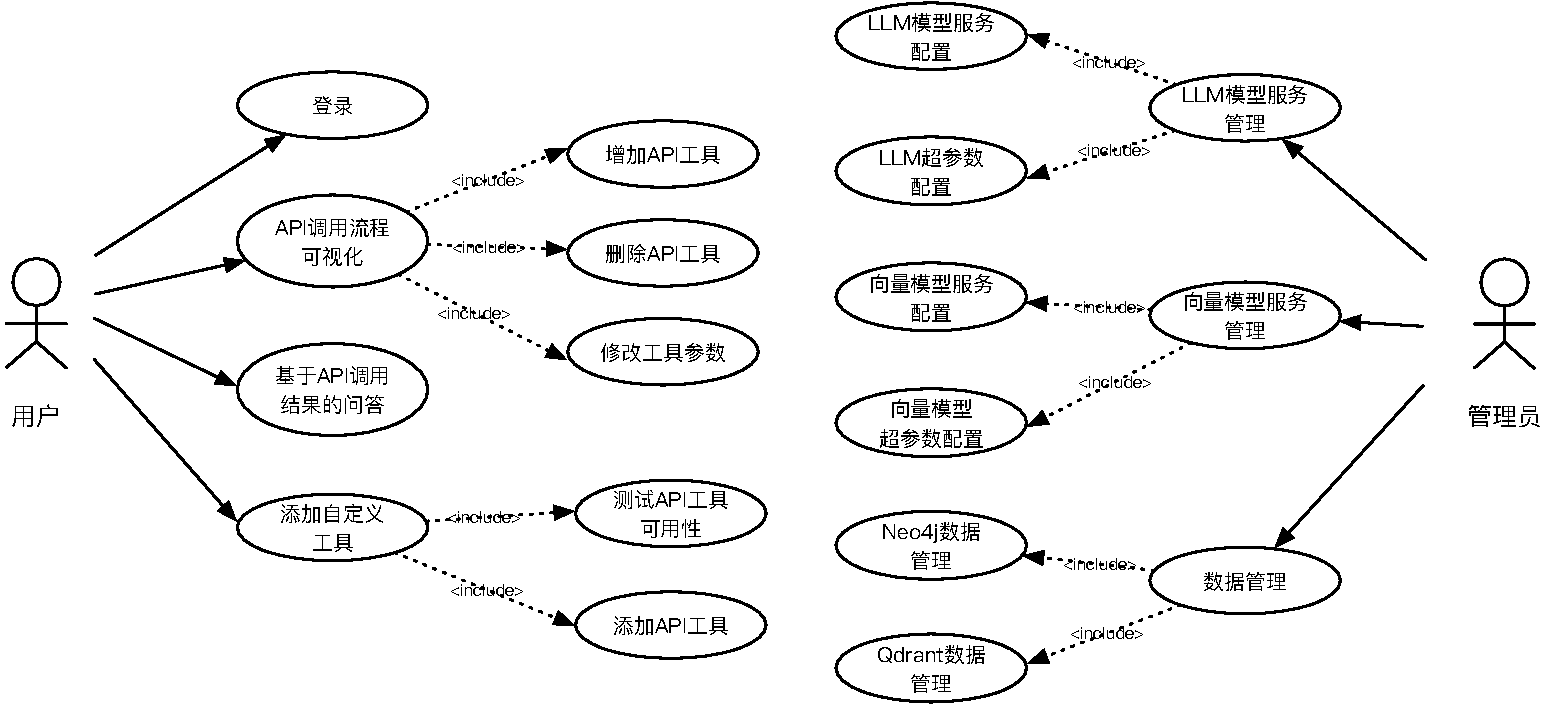
\includegraphics[height=6cm]{../assets/ch5-用例图.pdf}
  \bicaption{系统用例图}{System Usecase Diagram}
  \label{fig:usecase}
\end{figure}

我们采用面向对象的需求分析方法,绘制了系统的用例图。在该用例图中,我们定义了两种主要角色:系统用户和管理人员。系统用户包含普通用户和开发者,而管理人员则具有更高权限的管理功能。这样的角色划分帮助系统满足不同用户的需求,支持工具调用、数据管理、模型管理等任务。根据需求分析,系统应具备以下核心功能模块:

1.	用户与权限管理:系统应提供用户注册、登录、身份验证和权限分配功能。系统用户可根据权限访问相应模块,而管理人员具有配置用户权限的能力,以保障系统安全性和合理性。

2.	API调用流程管理与问答支持:系统支持用户通过可视化界面查看并编辑API调用流程,并能基于调用结果进行问答。API调用流程管理模块可展示调用步骤、输入输出等信息,用户可根据需要进行简单调整。问答模块则负责对编排好的工具流程进行调用和解析,生成总结性描述或回答用户问题。

3.	自定义工具与工具库管理:系统支持用户根据需求添加自定义工具,丰富工具库的扩展性。用户通过填写工具的配置信息并测试后,系统将自动集成到工具库,供用户选择和调用。同时,工具库还提供常用工具模板,方便用户浏览和直接调用。

4.	模型服务管理:系统为管理人员提供大语言模型和向量模型服务的管理功能。该模块支持模型的配置、更新和监控,以满足多种任务需求并优化系统性能。管理人员可以根据需要对模型进行更新,以确保系统提供高效的模型服务。

5. 数据库管理:系统应提供高效的图数据库和向量数据库管理功能,以支持管理员对不同类型的数据进行配置和管理。对于图数据库管理,平台应支持Neo4j等图数据库的配置,允许管理员查看数据库状态、管理数据结构和优化查询性能,以确保关系数据的高效存储和检索。对于向量数据库管理,平台应支持Qdrant等向量数据库的配置,允许管理员调整存储策略和搜索参数,以优化向量数据的存储和检索性能。系统支持大规模向量数据的导入、分片配置和索引更新,确保能够高效完成相似度计算,满足推荐系统和语义搜索等场景的需求。

\section{交互方案设计}

图~\ref{fig:system}为该系统的交互设计图。

\begin{figure}[!htp]
    \vspace{1em}
    \centering
    \setlength{\abovecaptionskip}{10pt} % 控制图片和caption之间的距离
    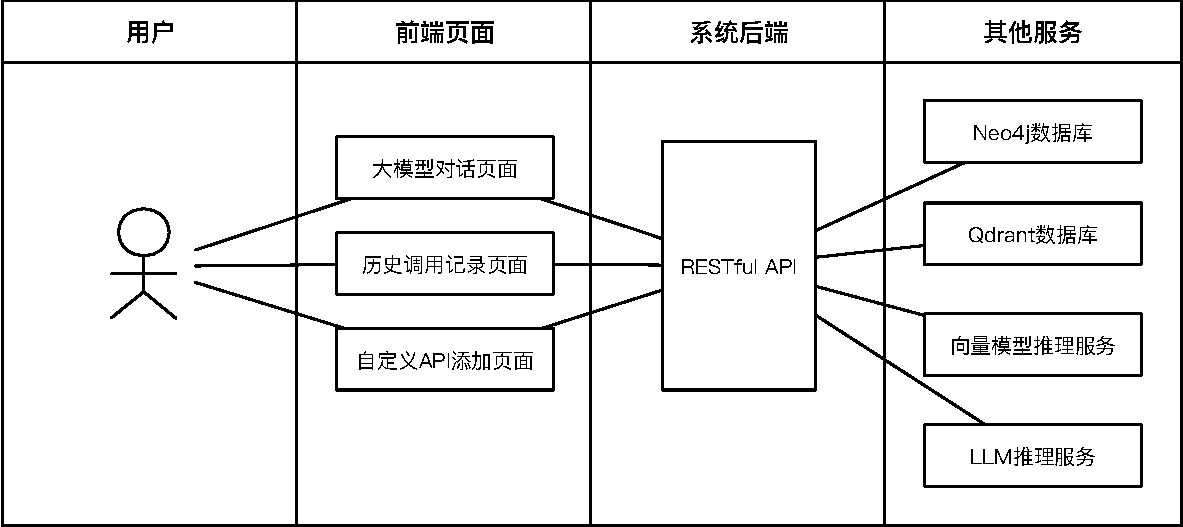
\includegraphics[height=5cm]{../assets/ch5-交互设计图.pdf}
    \bicaption{系统交互图}{System Usecase Diagram}
    \label{fig:interaction}
  \end{figure}


本系统主要有以下三个部分,前端交互界面、系统后端和其他服务模块,集成了不同模型的调用接口以及知识图谱查询功能,为用户提供了低门槛、用户友好的界面,支持用户通过自然语言的方式进行交互和提问。整体交互流程如图6.2所示:

	1.	前端页面:前端页面为用户提供了交互界面,支持大模型对话、历史调用记录以及自定义API工具添加等功能。用户可以通过这些页面与系统进行自然语言交互,例如通过对话界面向大模型提问、查看历史调用模板获取API使用信息,或在自定义页面添加新的API工具以扩展系统功能。
	2.	系统后端:系统后端作为核心控制层,通过RESTful API接口将前端用户请求传递至其他服务模块,并负责业务逻辑的处理。后端系统不仅管理用户请求的权限和数据存储,还充当API编排的核心,确保前端请求的安全性和规范性。在与其他服务模块的交互中,后端可以灵活调用图数据库、向量数据库以及模型推理服务,实现对知识图谱的查询和不同模型的协同调用,以满足复杂的查询和推理需求。
	3.	其他服务模块:其他服务模块包括Neo4j图数据库、Qdrant向量数据库、向量模型推理服务和LLM(大语言模型)推理服务。这些模块分别用于存储和查询图数据库、管理和检索向量化数据、支持基于向量相似度的搜索需求,以及提供大语言模型的对话和推理功能。系统后端根据用户需求对这些服务进行编排调用,确保用户问题得到高效而准确的解答。

通过以上三部分的协同工作,系统能够为用户提供全面的API编排调用智能问答、历史调用模板查询和自定义工具配置等服务,满足用户的需求,并提供了易用、易扩展的系统和良好的交互体验。

\section{系统架构设计}

图~\ref{fig:system}为该系统的系统软件架构设计图。

\begin{figure}[!htp]
    \vspace{1em}
    \centering
    \setlength{\abovecaptionskip}{10pt} % 控制图片和caption之间的距离
    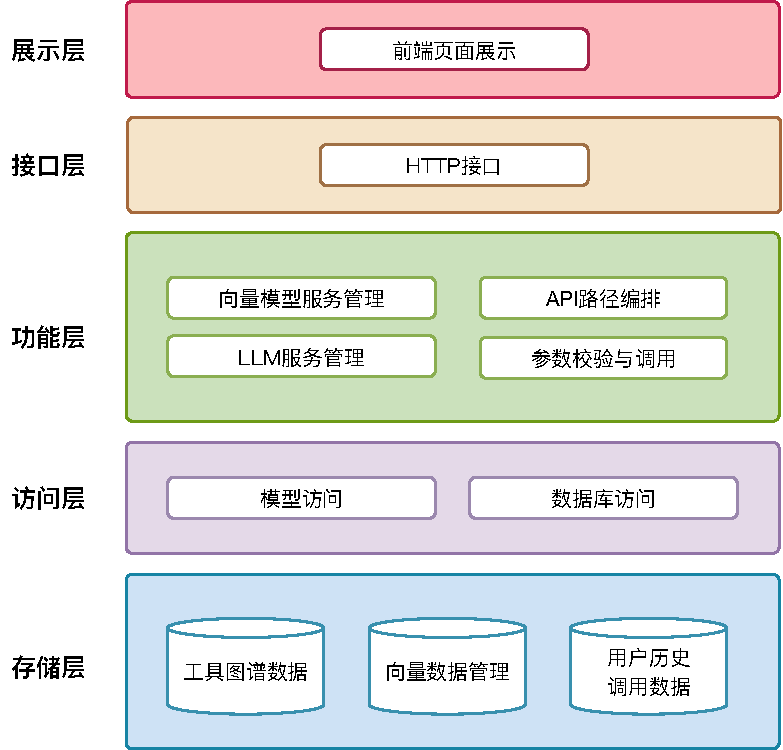
\includegraphics[height=8cm]{../assets/ch5-系统架构图.pdf}
    \bicaption{系统用例图}{System Usecase Diagram}
    \label{fig:system}
  \end{figure}

\subsection{存储层}
数据管理层主要负责下列内容的存储:
\begin{enumerate}
    \item API知识图谱的存储
    \item 向量形式存储的API详细信息,这些预先计算并存储在向量数据库中,便于快速计算
    \item 系统使用过程中的历史推理轨迹的存储,作为经验数据供后续参考
\end{enumerate}

\subsection{访问层}

负责数据的访问,包括对图数据库、向量数据库的访问和JSON格式的文件访问。封装了对存储层的访问,提供方便的数据访问接口,以便于功能层调用。

\subsection{功能层}
API编排层主要实现本系统的动态API编排功能。该层主要包括以下几个部分:
\begin{enumerate}
    \item \textbf{用户需求拆解模块}:通过大语言模型智能体机制,将用户的复杂、完整需求拆解为多个子需求,并对子需求逐一调用。
    \item \textbf{API推理轨迹检索模块}:根据子任务的任务描述,检索历史推理轨迹中相似任务,提供参考。
    \item \textbf{API知识图谱检索模块}:根据不同的检索模式,搜索API节点及相关信息作为返回。
    \item \textbf{基于图谱的DFS动态编排算法模块}:在知识图谱上进行搜索和回溯,得到最终的调用路径。
    \item \textbf{API参数获取模块}: 首先,我们获取得到对应API的参数信息以及用户的具体需求,提供给大语言模型让模型给出API所需的输入参数。
    \item \textbf{API调用模块}: 在该部分,会使用API参数获取模块的参数作为API输入来调用工具API,若执行成功则将JSON格式的调用结果传递到API调用结果总结模块。该部分设置了自动重试机制,若调用失败则自动重试3次,如果3次都失败则返回错误信息。
    \item \textbf{API调用结果总结模块}: 在执行并得到了API的调用结果后,将所有的API执行结果转化为自然语言的格式,将这些执行结果和用户原需求输入基于大语言模型的总结模块获取最终自然语言格式的总结内容。
\end{enumerate}

\subsection{接口层}

接口层负责提供对各种功能的访问接口,采用的是HTTP接口的形式。系统后端通过提供RESTful API格式的HTTP接口来供前端调用和访问。模型服务与平台后端也是用过HTTP接口来实现高效、安全的通信。

\subsection{展示层}
UI层是web前端页面,负责与用户直接交互,提供用户友好的界面。不同页面对应不同功能:
\begin{itemize}
    \item \textbf{信息问答页面}:用户通过自然语言输入具体的需求,然后系统会进行API调用路径的编排并依次调用,最终将总结好的自然语言文本的结果也提供给用户。整体的交互方式与大模型多轮对话是相似的。
    \item \textbf{自定义API添加页面}:用户可以通过填写API的详细信息,如API的名称、API的调用链接、API的具体参数类型和参数描述信息等添加新的API。添加新API后还需要经过测试,确保API调用的有效性再添加到API仓库中。
    \item \textbf{API历史调用参考页面}:用户可以可视化的形式浏览历史API调用记录,并通过选择和配置参数的方式再次调用历史API调用链。
\end{itemize}


\section{模块设计}

图xx展示了系统详细的功能层次结构。本系统的详细功能主要包含:用户验证、数据管理、模型服务管理、API工作流编排、API调用问答、自定义API存储。

\subsection{用户验证}
用户验证模块用于实现面向用户的API调用历史记录和模板库构建。该模块包含用户注册和登录功能,允许用户通过注册获得个人账号并登录系统使用。

\subsection{数据管理}
数据管理模块用于管理系统中的各类数据,包括知识图谱数据、API信息向量以及用户交互过程中的历史需求、API编排和调用结果等。主要存储在neo4j和Qdrant向量数据库中。

\subsection{模型服务管理}
模型服务管理模块包括模型接口封装和模型超参数配置功能。封装不同模型的调用代码为统一接口,对系统其他部分隐藏模型的具体细节。超参数配置则管理模型调用时的参数,如温度系数、最大长度、top\_k、top\_p等。

\subsection{API工作流编排}
API工作流编排模块包含以下三个子模块:
\begin{itemize}
    \item \textbf{编排模式选择}:提供用户可配置的编排选项。
    \item \textbf{编排结果展示}:通过可编辑任务框展示API编排结果,任务框中展示API名称、描述、参数等信息。
    \item \textbf{API流程自定义}:允许用户在生成的API流程基础上,进行增加、删除或修改,支持更灵活的API调用。
\end{itemize}

\subsection{API调用问答}
API调用问答模块通过流式输出和多轮交互,提升用户体验。流式输出模块增强用户等待结果时的体验,多轮交互模块保存上下文中的API调用结果,支持进一步提问。

\subsection{自定义API存储}
自定义API存储模块通过API添加和测试模块,支持用户将自定义API添加到系统中,提高系统扩展性和可用性。

\section{系统实现}

本节将会介绍系统的实现方法。首先是技术选型方面,考虑到与大语言模型、深度学习有关的代码都采用Python编写,我们也采用了Python技术栈。
我们采用了前后端分离的方式,选择了FastAPI作为后端框架,前后端之间通过HTTP接口进行网络通信。
在前端页面部分,我们选用了目前大语言模型Chatbot有关最流行的前端框架之一,Streamlit前端框架来实现。



\section{本章小结}